\documentclass[]{book}
\usepackage{lmodern}
\usepackage{amssymb,amsmath}
\usepackage{ifxetex,ifluatex}
\usepackage{fixltx2e} % provides \textsubscript
\ifnum 0\ifxetex 1\fi\ifluatex 1\fi=0 % if pdftex
  \usepackage[T1]{fontenc}
  \usepackage[utf8]{inputenc}
\else % if luatex or xelatex
  \ifxetex
    \usepackage{mathspec}
  \else
    \usepackage{fontspec}
  \fi
  \defaultfontfeatures{Ligatures=TeX,Scale=MatchLowercase}
\fi
% use upquote if available, for straight quotes in verbatim environments
\IfFileExists{upquote.sty}{\usepackage{upquote}}{}
% use microtype if available
\IfFileExists{microtype.sty}{%
\usepackage[]{microtype}
\UseMicrotypeSet[protrusion]{basicmath} % disable protrusion for tt fonts
}{}
\PassOptionsToPackage{hyphens}{url} % url is loaded by hyperref
\usepackage[unicode=true]{hyperref}
\hypersetup{
            pdftitle={PSY6422 Data Management and Visualisation @ The University of Sheffield},
            pdfauthor={Tom Stafford},
            pdfborder={0 0 0},
            breaklinks=true}
\urlstyle{same}  % don't use monospace font for urls
\usepackage{natbib}
\bibliographystyle{apalike}
\usepackage{color}
\usepackage{fancyvrb}
\newcommand{\VerbBar}{|}
\newcommand{\VERB}{\Verb[commandchars=\\\{\}]}
\DefineVerbatimEnvironment{Highlighting}{Verbatim}{commandchars=\\\{\}}
% Add ',fontsize=\small' for more characters per line
\usepackage{framed}
\definecolor{shadecolor}{RGB}{248,248,248}
\newenvironment{Shaded}{\begin{snugshade}}{\end{snugshade}}
\newcommand{\KeywordTok}[1]{\textcolor[rgb]{0.13,0.29,0.53}{\textbf{#1}}}
\newcommand{\DataTypeTok}[1]{\textcolor[rgb]{0.13,0.29,0.53}{#1}}
\newcommand{\DecValTok}[1]{\textcolor[rgb]{0.00,0.00,0.81}{#1}}
\newcommand{\BaseNTok}[1]{\textcolor[rgb]{0.00,0.00,0.81}{#1}}
\newcommand{\FloatTok}[1]{\textcolor[rgb]{0.00,0.00,0.81}{#1}}
\newcommand{\ConstantTok}[1]{\textcolor[rgb]{0.00,0.00,0.00}{#1}}
\newcommand{\CharTok}[1]{\textcolor[rgb]{0.31,0.60,0.02}{#1}}
\newcommand{\SpecialCharTok}[1]{\textcolor[rgb]{0.00,0.00,0.00}{#1}}
\newcommand{\StringTok}[1]{\textcolor[rgb]{0.31,0.60,0.02}{#1}}
\newcommand{\VerbatimStringTok}[1]{\textcolor[rgb]{0.31,0.60,0.02}{#1}}
\newcommand{\SpecialStringTok}[1]{\textcolor[rgb]{0.31,0.60,0.02}{#1}}
\newcommand{\ImportTok}[1]{#1}
\newcommand{\CommentTok}[1]{\textcolor[rgb]{0.56,0.35,0.01}{\textit{#1}}}
\newcommand{\DocumentationTok}[1]{\textcolor[rgb]{0.56,0.35,0.01}{\textbf{\textit{#1}}}}
\newcommand{\AnnotationTok}[1]{\textcolor[rgb]{0.56,0.35,0.01}{\textbf{\textit{#1}}}}
\newcommand{\CommentVarTok}[1]{\textcolor[rgb]{0.56,0.35,0.01}{\textbf{\textit{#1}}}}
\newcommand{\OtherTok}[1]{\textcolor[rgb]{0.56,0.35,0.01}{#1}}
\newcommand{\FunctionTok}[1]{\textcolor[rgb]{0.00,0.00,0.00}{#1}}
\newcommand{\VariableTok}[1]{\textcolor[rgb]{0.00,0.00,0.00}{#1}}
\newcommand{\ControlFlowTok}[1]{\textcolor[rgb]{0.13,0.29,0.53}{\textbf{#1}}}
\newcommand{\OperatorTok}[1]{\textcolor[rgb]{0.81,0.36,0.00}{\textbf{#1}}}
\newcommand{\BuiltInTok}[1]{#1}
\newcommand{\ExtensionTok}[1]{#1}
\newcommand{\PreprocessorTok}[1]{\textcolor[rgb]{0.56,0.35,0.01}{\textit{#1}}}
\newcommand{\AttributeTok}[1]{\textcolor[rgb]{0.77,0.63,0.00}{#1}}
\newcommand{\RegionMarkerTok}[1]{#1}
\newcommand{\InformationTok}[1]{\textcolor[rgb]{0.56,0.35,0.01}{\textbf{\textit{#1}}}}
\newcommand{\WarningTok}[1]{\textcolor[rgb]{0.56,0.35,0.01}{\textbf{\textit{#1}}}}
\newcommand{\AlertTok}[1]{\textcolor[rgb]{0.94,0.16,0.16}{#1}}
\newcommand{\ErrorTok}[1]{\textcolor[rgb]{0.64,0.00,0.00}{\textbf{#1}}}
\newcommand{\NormalTok}[1]{#1}
\usepackage{longtable,booktabs}
% Fix footnotes in tables (requires footnote package)
\IfFileExists{footnote.sty}{\usepackage{footnote}\makesavenoteenv{long table}}{}
\usepackage{graphicx,grffile}
\makeatletter
\def\maxwidth{\ifdim\Gin@nat@width>\linewidth\linewidth\else\Gin@nat@width\fi}
\def\maxheight{\ifdim\Gin@nat@height>\textheight\textheight\else\Gin@nat@height\fi}
\makeatother
% Scale images if necessary, so that they will not overflow the page
% margins by default, and it is still possible to overwrite the defaults
% using explicit options in \includegraphics[width, height, ...]{}
\setkeys{Gin}{width=\maxwidth,height=\maxheight,keepaspectratio}
\IfFileExists{parskip.sty}{%
\usepackage{parskip}
}{% else
\setlength{\parindent}{0pt}
\setlength{\parskip}{6pt plus 2pt minus 1pt}
}
\setlength{\emergencystretch}{3em}  % prevent overfull lines
\providecommand{\tightlist}{%
  \setlength{\itemsep}{0pt}\setlength{\parskip}{0pt}}
\setcounter{secnumdepth}{5}
% Redefines (sub)paragraphs to behave more like sections
\ifx\paragraph\undefined\else
\let\oldparagraph\paragraph
\renewcommand{\paragraph}[1]{\oldparagraph{#1}\mbox{}}
\fi
\ifx\subparagraph\undefined\else
\let\oldsubparagraph\subparagraph
\renewcommand{\subparagraph}[1]{\oldsubparagraph{#1}\mbox{}}
\fi

% set default figure placement to htbp
\makeatletter
\def\fps@figure{htbp}
\makeatother

\usepackage{booktabs}

\newenvironment{danger}
    {
    \hline\\
    }
    { 
    \\\\\hline
    }
    
\newenvironment{warning}
    {
    \hline\\
    }
    { 
    \\\\\hline
    }
    
\newenvironment{info}
    {
    \hline\\
    }
    { 
    \\\\\hline
    }
    
\newenvironment{try}
    {
    \hline\\
    }
    { 
    \\\\\hline
    }

\title{PSY6422 Data Management and Visualisation @ The University of Sheffield}
\author{Tom Stafford}
\date{2020-04-21}

\begin{document}
\maketitle

{
\setcounter{tocdepth}{1}
\tableofcontents
}
\chapter{Module Overview}\label{module-overview}

PSY6422 Data Management and Visualisation is part of the MSc in
Psychological Research Methods with Data Science taught at The
University of Sheffield by
\href{http://tomstafford.staff.shef.ac.uk/}{Tom Stafford}

\emph{Note this is a placeholder page. In 2020 most of this material was
delivered offline. I am adding notes online as I can, so these pages in
particular may evolve quickly}

\section{Motivation}\label{motivation}

You are aiming to produce reproducible workflows - scripts that automate
all steps between raw data and the final data in your papers.

Point and click solutions (spreedsheets, SPSS) are inadequate.

As well as being \emph{reproducible} (by you or other researchers) your
work should be \emph{legible} (to Future You, or other researchers) and
\emph{scalable} (it should work as well on 400,000 data points as on
40).

You will need help to do this. Therefore you will use Open Source
solutions - these are analysis products which have a worldwide community
of people using them, and the infrastructure which supports sharing
advice and solutions.

In practice, this means you are going to start by using R (you could use
\href{https://tomstafford.github.io/psy6422/appendices.html\#python}{Python},
but this module is based on R)

\section{Resources for current
students}\label{resources-for-current-students}

\href{https://drive.google.com/drive/folders/1tuaTS6RPYOXh-XByRffFS1FDzbvvFs_w}{Google
Drive} (UoS login required to access):

Includes slides and workbooks, as well as these specific documents

\begin{itemize}
\tightlist
\item
  \href{https://docs.google.com/spreadsheets/d/1fyvjYhai6nIaOUymkUrlGIXL89cG76lI8bLXirPbaOw/edit?usp=drivesdk}{Timetable}
\item
  \href{https://docs.google.com/document/d/1kEDLaELoFyRBCsQLkZZP1PNbNaw2uUM6AAQhd42ExwQ/edit?usp=drivesdk}{Useful
  information}
\item
  \href{https://docs.google.com/spreadsheets/d/1DS91tnTtC8qPQHchAbzkOK57vvsSLIQc9FN3nPp9bQY/edit?usp=drivesdk}{Assessment
  Criteria}
\end{itemize}

And of course these pages (hosted on github, no login required)

You may particularly enjoy the \href{extra-reading.html}{Reading list}

\section{Course Outline}\label{course-outline}

In 2020 we are covering a compressed curriculum. The topics we cover
are:

\begin{enumerate}
\def\labelenumi{\arabic{enumi}.}
\tightlist
\item
  Module overview - ethics and aesthetics of visualisaion, the
  importance of reproducible workflows
\item
  Project organisation - fundamentals of data storage, syncronisation
  and sharing
\item
  R / Rstudio - introduction to the statistical computing language
\item
  Making graphs
\item
  Data Management
\item
  Data Management 2
\item
  Coding principles - fundamental principles of coding, writing good
  code, asking for help
\item
  Rmarkdown
\item
  Git and github
\item
  Publishing to pages - like this one!
\item
  Advanced topics
\end{enumerate}

Stretch goals:

Unfortunately we won't have time this year for a number of advanced
topics which I would like to cover. Hopefully next year:

\begin{itemize}
\tightlist
\item
  Jupyter notebooks
\item
  The terminal / ssh
\item
  Interactive visualisation with Shiny apps
\item
  SQL
\end{itemize}

\section{Example Projects}\label{example-projects}

The bulk of the assessment is to conduct and publish your own analysis
project. Here is an example small project which gives an idea of what I
mean

\begin{itemize}
\tightlist
\item
  SuperTues: \href{https://tomstafford.github.io/supertues/}{Published},
  \href{https://github.com/tomstafford/supertues}{repo}
\end{itemize}

Stretch goal is to build an interactive data visualisation using Shiny

\begin{itemize}
\tightlist
\item
  Here's one I built earlier
  \href{https://sheffield-university.shinyapps.io/decision_power/}{Power
  analyser}
\end{itemize}

\section{More}\label{more}

\begin{itemize}
\tightlist
\item
  Russ Poldrack's
  \href{http://www.russpoldrack.org/2016/05/advice-for-learning-to-code-from-scratch.html}{Advice
  for learning to code from scratch}
\end{itemize}

\chapter{Project Organisation}\label{project-organisation}

This is a placeholder page. This material was delivered offline

Specific resources:

\begin{quote}
\begin{quote}
TO APPEAR\textless{}\textless{}
\end{quote}
\end{quote}

\section{Data Management}\label{data-management}

Everything recorded during an experiment, whether by you or the
computer, is data. All log files. Everything.

Never delete \emph{any} data.

All data should be backed-up automatically. Any back up process which
requires you to remember to deploy it is fragile. Use a cloud
synchronisation service like Google Drive or Dropbox.

Never edit the raw data files. They should exist is a folder called
\raw or \data and only ever be opened, never modified in any way

\section{Reading:}\label{reading}

\begin{itemize}
\tightlist
\item
  \href{http://vita.had.co.nz/papers/tidy-data.pdf}{Tidy Data
  organisation}
\item
  \href{http://bayesfactor.blogspot.co.uk/2015/11/habits-and-open-data-helping-students.html}{Habits
  and open data: Helping students develop a theory of scientific mind}
\item
  Broman \& Woo (2017)
  \href{https://www.tandfonline.com/doi/full/10.1080/00031305.2017.1375989}{Data
  Organization in Spreadsheets}
\end{itemize}

\chapter{R \& R Studio}\label{r-r-studio}

This is a placeholder page. This material was delivered offline

Specific resources:

\begin{quote}
\begin{quote}
TO APPEAR\textless{}\textless{}
\end{quote}
\end{quote}

\chapter{Making Graphs}\label{making-graphs}

This is a placeholder page. This material was delivered offline

Specific resources:

\begin{quote}
\begin{quote}
TO APPEAR\textless{}\textless{}
\end{quote}
\end{quote}

\chapter{Data Management}\label{data-management-1}

This is a placeholder page. This material was delivered offline

Specific resources:

\begin{quote}
\begin{quote}
TO APPEAR\textless{}\textless{}
\end{quote}
\end{quote}

\chapter{Coding Principles}\label{coding-principles}

This class is about two kinds of fundamental principles of coding. The
first is fundamental methods of making code do what you want - if
statement, loops, functions. The second is fundamental principles of
good code. Although we are using R, all programming languages use
similar methods (although the exact syntax differs), and the principles
of good code will also apply across languages.

As well demonstrating these fundamentals, these pages also introduce the
vocabulary used to discuss them. Knowing the vocabulary helps because it
means you know what terms to use when searching for solutions to
problems you have.

\section{Fundamental methods}\label{fundamental-methods}

\begin{enumerate}
\def\labelenumi{\arabic{enumi}.}
\tightlist
\item
  \protect\hyperlink{if}{if statements}
\item
  \protect\hyperlink{loops}{loops}
\item
  \protect\hyperlink{functions}{functions}
\end{enumerate}

\hypertarget{if}{\subsection{If statements}\label{if}}

So far we have written simple scripts that do things in order, top to
bottom

\begin{Shaded}
\begin{Highlighting}[]
\NormalTok{a <-}\StringTok{ }\DecValTok{1} \CommentTok{# define a variable}
\NormalTok{a <-}\StringTok{ }\NormalTok{a }\OperatorTok{+}\StringTok{ }\DecValTok{1} \CommentTok{#add 1}
\KeywordTok{print}\NormalTok{(a) }\CommentTok{# output the result}
\end{Highlighting}
\end{Shaded}

\begin{verbatim}
## [1] 2
\end{verbatim}

The first block above is the code, the second block (the lines which
start with \texttt{\#\#}) is the output.

Changing which statements are run is called ``flow control''. An ``If
statement'' is a fundamental way of doing this. It allows us to specify
one set statements to run if a certain conditions is met. For example

\begin{Shaded}
\begin{Highlighting}[]
\NormalTok{a <-}\StringTok{ }\DecValTok{1} \CommentTok{# define a variable}
\NormalTok{a <-}\StringTok{ }\NormalTok{a }\OperatorTok{+}\StringTok{ }\DecValTok{1} \CommentTok{#add 1}
\ControlFlowTok{if}\NormalTok{(a}\OperatorTok{>}\DecValTok{4}\NormalTok{) }\CommentTok{# this is the condition which has to be met, the 'test expression'}
\NormalTok{  \{}\KeywordTok{print}\NormalTok{(a)\} }\CommentTok{# this statement runs if the test expression is true}
\end{Highlighting}
\end{Shaded}

Notice there is no output. Copy the code to your own computer and run
it. Now change the first line to \texttt{a\ \textless{}-\ 9} and run it
again.

An If statement defines a branch in the flow of a script. The default
can be nothing happening, but sometimes you want to define two
alternatives. You can do this with an
``If\ldots{}else\ldots{}statement''

\begin{Shaded}
\begin{Highlighting}[]
\NormalTok{a <-}\StringTok{ }\DecValTok{1} \CommentTok{# define a variable}
\NormalTok{a <-}\StringTok{ }\NormalTok{a }\OperatorTok{+}\StringTok{ }\DecValTok{1} \CommentTok{#add 1}
\ControlFlowTok{if}\NormalTok{(a}\OperatorTok{>}\DecValTok{4}\NormalTok{)\{ }\CommentTok{# this is the condition which has to be met, the 'test expression'}
  \KeywordTok{print}\NormalTok{(}\KeywordTok{paste}\NormalTok{(a,}\StringTok{" is more than 4"}\NormalTok{)) }\CommentTok{# this statement runs if the test expression is true}
\NormalTok{\} }\ControlFlowTok{else}\NormalTok{ \{}
\NormalTok{  \{}\KeywordTok{print}\NormalTok{(}\KeywordTok{paste}\NormalTok{(a,}\StringTok{" is equal or less than 4"}\NormalTok{))\} }\CommentTok{# this statement runs if the test expression is false}
\NormalTok{\}}
\end{Highlighting}
\end{Shaded}

\begin{verbatim}
## [1] "2  is equal or less than 4"
\end{verbatim}

You can actually have as many branches as you like, defining a series of
test\_expressions, like this

\begin{Shaded}
\begin{Highlighting}[]
\NormalTok{type_of_thing=}\StringTok{''} 
\KeywordTok{print}\NormalTok{(}\StringTok{"Is four a lot?"}\NormalTok{)}
\ControlFlowTok{if}\NormalTok{ (type_of_thing}\OperatorTok{==}\StringTok{'Murders'}\NormalTok{)\{}
  \KeywordTok{print}\NormalTok{(}\StringTok{"yes"}\NormalTok{)}
\NormalTok{\} }\ControlFlowTok{else} \ControlFlowTok{if}\NormalTok{ (type_of_thing}\OperatorTok{==}\StringTok{'Dollars'}\NormalTok{)\{}
  \KeywordTok{print}\NormalTok{(}\StringTok{"no"}\NormalTok{)}
\NormalTok{\} }\ControlFlowTok{else}\NormalTok{ \{}
  \KeywordTok{print}\NormalTok{(}\StringTok{"Depends on the context"}\NormalTok{)}
\NormalTok{\}}
\end{Highlighting}
\end{Shaded}

\begin{verbatim}
## [1] "Is four a lot?"
## [1] "Depends on the context"
\end{verbatim}

\hypertarget{loops}{\subsection{Loops}\label{loops}}

Loops repeat, either iterating over a set values, like this:

\texttt{r\ \ \ for\ (i\ in\ 1:5)\{\ \ \ print(i)\ \ \ \}}

\texttt{\#\#\ {[}1{]}\ 1\ \ \ \#\#\ {[}1{]}\ 2\ \ \ \#\#\ {[}1{]}\ 3\ \ \ \#\#\ {[}1{]}\ 4\ \ \ \#\#\ {[}1{]}\ 5}

Or until some condition is met

\begin{Shaded}
\begin{Highlighting}[]
\NormalTok{i <-}\StringTok{ }\DecValTok{1} \CommentTok{#need to initialise a starting value}
\ControlFlowTok{while}\NormalTok{(i}\OperatorTok{<}\DecValTok{6}\NormalTok{)\{}
  \KeywordTok{print}\NormalTok{(i)}
\NormalTok{  i <-}\StringTok{ }\NormalTok{i }\OperatorTok{+}\StringTok{ }\DecValTok{1} \CommentTok{# increment the value of the counter}
\NormalTok{\}}
\end{Highlighting}
\end{Shaded}

\begin{verbatim}
## [1] 1
## [1] 2
## [1] 3
## [1] 4
## [1] 5
\end{verbatim}

Note that this second version, a ``while loop'' uses a test expression
just like an if statement

Loops are useful wherever you might want to repeat some operation.

\begin{Shaded}
\begin{Highlighting}[]
\NormalTok{years <-}\StringTok{ }\DecValTok{10} \CommentTok{#how many years since you started saving}
\NormalTok{savings <-}\DecValTok{100} \CommentTok{#how much you start with}
\NormalTok{interest <-}\StringTok{ }\FloatTok{1.05} \CommentTok{#rate of interest, ie 5% interest}
\CommentTok{#Calculate using a loop}
\ControlFlowTok{for}\NormalTok{ (years }\ControlFlowTok{in} \DecValTok{1}\OperatorTok{:}\NormalTok{years)\{}
\NormalTok{  savings<-savings}\OperatorTok{*}\NormalTok{interest}
\NormalTok{\}}
\KeywordTok{print}\NormalTok{(}\KeywordTok{paste}\NormalTok{(}\StringTok{"After"}\NormalTok{, years, }\StringTok{"years you will have £"}\NormalTok{, }\KeywordTok{round}\NormalTok{(savings,}\DecValTok{2}\NormalTok{))) }\CommentTok{#save more, kids}
\end{Highlighting}
\end{Shaded}

\begin{verbatim}
## [1] "After 10 years you will have £ 162.89"
\end{verbatim}

Lots of people advise against using loops because they are can be slow
and it isn't always obvious what they are doing. Alternatives often
exist, like vectorisation:

\begin{Shaded}
\begin{Highlighting}[]
\NormalTok{years <-}\StringTok{ }\DecValTok{20} \CommentTok{#how many years since you started saving}
\NormalTok{savings <-}\DecValTok{100} \CommentTok{#how much you start with}
\NormalTok{interest <-}\StringTok{ }\FloatTok{1.05} \CommentTok{#rate of interest, ie 5% interest}
\CommentTok{#Calculate using a vector}
\NormalTok{total_at_each_year=savings}\OperatorTok{*}\NormalTok{interest}\OperatorTok{**}\NormalTok{(}\DecValTok{1}\OperatorTok{:}\NormalTok{years) }\CommentTok{#rather than a loop all the answer values are stored in a single vector}
\CommentTok{#plot(total_at_each_year,xlab="years") #bonus! We can plot, since we now have all the intervening values saved}
\end{Highlighting}
\end{Shaded}

The problem is, loops are the natural way to think about some problems.
Often I first write my code with loops then, when I know what I really
want to do I try and work out a way to do it with vectorisation.

\hypertarget{functions}{\subsection{Functions}\label{functions}}

Functions take in values (called ``arguments''), do something with them,
and give a value or values back in return. You have already used
functions, for example the mean function

\begin{Shaded}
\begin{Highlighting}[]
\NormalTok{my_nums=}\KeywordTok{c}\NormalTok{(}\DecValTok{78}\NormalTok{,}\DecValTok{12}\NormalTok{,}\DecValTok{32}\NormalTok{,}\DecValTok{24}\NormalTok{,}\DecValTok{03}\NormalTok{,}\DecValTok{89}\NormalTok{) }\CommentTok{#just a vector of some numbers}
\KeywordTok{mean}\NormalTok{(my_nums) }\CommentTok{#use the mean function to find the average}
\end{Highlighting}
\end{Shaded}

\begin{verbatim}
## [1] 39.66667
\end{verbatim}

Functions always do the same thing, but give different results depending
on the inputs (depending on the ``arguments you pass to the function'').

You can write your own functions, and then use them again and again
(``call them again and again''). Here is the general form of a function

\begin{Shaded}
\begin{Highlighting}[]
\NormalTok{myfunctionname <-}\StringTok{ }\ControlFlowTok{function}\NormalTok{(input_value) \{}
\CommentTok{# comment line helpfully explaining what the function does}
\NormalTok{output_value <-}\StringTok{ }\NormalTok{input_value }\CommentTok{#lines of code which do something to the input to produce the output}
\KeywordTok{return}\NormalTok{(output_value)}
\NormalTok{\}}
\end{Highlighting}
\end{Shaded}

Note a couple of things: when you run this code it does not produce any
output, but a new object appears in the ``global environment'' window,
top right. Like a variable, your function is now stored in the memory of
the current R session.

You can call this function now. If you close R you'll need to define the
function again by running the above code again (other functions are
inbuilt, like \texttt{mean} and are loaded at startup, or when you use
the \texttt{library} command to load a set of functions).

Now, when we call the function, we pass actual values.

\begin{Shaded}
\begin{Highlighting}[]
\KeywordTok{myfunctionname}\NormalTok{(}\DecValTok{3}\NormalTok{)}
\end{Highlighting}
\end{Shaded}

\begin{verbatim}
## [1] 3
\end{verbatim}

Let's make our a slightly more complicated

\begin{Shaded}
\begin{Highlighting}[]
\NormalTok{outcheck <-}\StringTok{ }\ControlFlowTok{function}\NormalTok{(val,threshold) \{}
\CommentTok{# outlier checker}
\ControlFlowTok{if}\NormalTok{(val}\OperatorTok{<}\NormalTok{threshold)\{}
\NormalTok{  output_value <-}\StringTok{ }\NormalTok{val }\CommentTok{#if value is below theshold return that value}
\NormalTok{\} }\ControlFlowTok{else}\NormalTok{ \{}
\NormalTok{  output_value <-}\StringTok{ }\OtherTok{NA} \CommentTok{#otherwise, return NaN}
\NormalTok{\}}
\KeywordTok{return}\NormalTok{(output_value)}
\NormalTok{\}}
\end{Highlighting}
\end{Shaded}

This function takes two input values, and returns a single value which
depends on the relation between the two

\begin{Shaded}
\begin{Highlighting}[]
\KeywordTok{outcheck}\NormalTok{(}\DecValTok{3}\NormalTok{,}\DecValTok{5}\NormalTok{)}
\end{Highlighting}
\end{Shaded}

\begin{verbatim}
## [1] 3
\end{verbatim}

\begin{Shaded}
\begin{Highlighting}[]
\KeywordTok{outcheck}\NormalTok{(}\DecValTok{7}\NormalTok{,}\DecValTok{5}\NormalTok{)}
\end{Highlighting}
\end{Shaded}

\begin{verbatim}
## [1] NA
\end{verbatim}

\subsubsection{A note about scope}\label{a-note-about-scope}

Variables within functions are kept `inside' the functions (within the
``scope'' of the function). Once you pass a value to a function is
acquires the label set in the function definition. Variables defined
within the function don't persist outside of it (they don't affect the
``global environment'')

So, for example, it doesn't matter if you have another variable called
\texttt{threshold}, the threshold within the function is set by the
second value passed it. Like this:

\begin{verbatim}
                                                                                                                                                                                                                                                            ```r
                                                                                                                                                                                                                                                                                                                                                                                                                                                                                                                          threshold <- 100
                                                                                                                                                                                                                                                                                                                                                                                                                                                                                                                          outcheck(7,5) #returns NA because 7 is higher than 5
                                                                                                                                                                                                                                                            ```
                                                                                                                                                                                                                                                            
                                                                                                                                                                                                                                                            ```
                                                                                                                                                                                                                                                            ## [1] NA
                                                                                                                                                                                                                                                            ```
                                                                                                                                                                                                                                                          
                                                                                                                                                                                                                                                          
                                                                                                                                                                                                                                                          ### Exercises
                                                                                                                                                                                                                                                          
                                                                                                                                                                                                                                                          * Write an if...else statement that prints "ODD" if the number is odd, "EVEN" if the number is even
                                                                                                                                                                                                                                                          * hint: you might use the remainder function %% (try 4%%2 to see how much is left when you divide 4 by 2)
                                                                                                                                                                                                                                                          * Write a loop which goes from 10 to 20 in steps of 3
                                                                                                                                                                                                                                                          * Write a function which prints "FIZZ" if a number is divisible by 3, and "BUZZ" if it is divisible by 5 and "FIZZBUZZ" if it is divisble by 3 *and* 5
                                                                                                                                                                                                                                                          * Write a loop which counts from 1 to 100 and applies the fizzbuzz function to each number
                                                                                                                                                                                                                                                          
                                                                                                                                                                                                                                                          
                                                                                                                                                                                                                                                          
                                                                                                                                                                                                                                                          ### More
                                                                                                                                                                                                                                                          
                                                                                                                                                                                                                                                          Lisa DeBruine, & Dale Barr. (2019, December 5). Data Skills for Reproducible Science (Version 1.0.0). Zenodo. http://doi.org/10.5281/zenodo.3564555: [Iterations & Functions](https://psyteachr.github.io/msc-data-skills/func.html)
                                                                                                                                                                                                                                                          
                                                                                                                                                                                                                                                          [datamentor.io on Flow control](https://www.datamentor.io/r-programming/if-else-statement/)
                                                                                                                                                                                                                                                          
                                                                                                                                                                                                                                                          ## Fundamental principles of good code
                                                                                                                                                                                                                                                          
                                                                                                                                                                                                                                                          ### Readability Matters
                                                                                                                                                                                                                                                          
                                                                                                                                                                                                                                                          Your most important collaborator is you from six months ago, and they don't answer email.
\end{verbatim}

Good code doesn't just work, it is easy to understand. This supports the
code being checked for errors, modified and improved (by you as well as
by other people).

\begin{verbatim}
                                                                                                                                                                                                                                                          To support this you should make your code readable. This means commenting your code, but also laying it out nicely, and using sensible names for variables and function. The aim is to make the code explain itself, as well as doing something. Someone who reads your code - a future you maybe, or a collaborator - needs to be able to run the code, yes, but they also need to know what you are doing and why you are doing. 
                                                                                                                                                                                                                                                          
                                                                                                                                                                                                                                                          Look at this function, it hard to understand, right?
                                                                                                                                                                                                                                                            
                                                                                                                                                                                                                                                            
                                                                                                                                                                                                                                                            
                                                                                                                                                                                                                                                            ```r
                                                                                                                                                                                                                                                                                                                                                                                                                                                                                                                          pf <- function(n){ p=1 ; if (n>1){ i = 2; while( (i<(n/2+1)) & (p==1) ) {if (n%%i ==0) p=0; i=i+1 }  } else {p=0 }; return(p) }
                                                                                                                                                                                                                                                            ```
                                                                                                                                                                                                                                                          
                                                                                                                                                                                                                                                          This kind of code is very compressed. You can fit a lot in a few lines, but it is useless because nobody else will understand it, and probably the person who wrote it won't understand it when they come back to it (and that means they will miss any bugs, or will find it hard to improve or repurpose).
\end{verbatim}

Readability is improved a lot by adding some spacing and tabs. Have
another go at figuring out what the code does:

\begin{Shaded}
\begin{Highlighting}[]
\NormalTok{pf <-}\StringTok{ }\ControlFlowTok{function}\NormalTok{(n)\{}
\NormalTok{  p=}\DecValTok{1}
  \ControlFlowTok{if}\NormalTok{ (n}\OperatorTok{>}\DecValTok{1}\NormalTok{)\{ }
\NormalTok{    i =}\StringTok{ }\DecValTok{2} 
      \ControlFlowTok{while}\NormalTok{( (i}\OperatorTok{<}\NormalTok{(n}\OperatorTok{/}\DecValTok{2}\OperatorTok{+}\DecValTok{1}\NormalTok{)) }\OperatorTok{&}\StringTok{ }\NormalTok{(p}\OperatorTok{==}\DecValTok{1}\NormalTok{) ) \{}
        \ControlFlowTok{if}\NormalTok{ (n}\OperatorTok\NormalTok{i }\OperatorTok{==}\DecValTok{0}\NormalTok{) \{}
\NormalTok{          p=}\DecValTok{0}
\NormalTok{        \}}
\NormalTok{        i=i}\OperatorTok{+}\DecValTok{1}
\NormalTok{      \}}
\NormalTok{  \} }\ControlFlowTok{else}\NormalTok{ \{}
\NormalTok{    p=}\DecValTok{0}
\NormalTok{  \}}
  \KeywordTok{return}\NormalTok{(p)}
\NormalTok{\}}
\end{Highlighting}
\end{Shaded}

Now we make the variable and function names sensible:

\begin{Shaded}
\begin{Highlighting}[]
\NormalTok{primecheck <-}\StringTok{ }\ControlFlowTok{function}\NormalTok{(num)\{}
\NormalTok{  isprime=}\OtherTok{TRUE}
  \ControlFlowTok{if}\NormalTok{ (num}\OperatorTok{>}\DecValTok{1}\NormalTok{)\{ }
\NormalTok{    i =}\StringTok{ }\DecValTok{2} 
      \ControlFlowTok{while}\NormalTok{( (i}\OperatorTok{<}\NormalTok{(num}\OperatorTok{/}\DecValTok{2}\OperatorTok{+}\DecValTok{1}\NormalTok{)) }\OperatorTok{&}\StringTok{ }\NormalTok{(isprime}\OperatorTok{==}\OtherTok{TRUE}\NormalTok{) ) \{}
        \ControlFlowTok{if}\NormalTok{ (num}\OperatorTok\NormalTok{i }\OperatorTok{==}\DecValTok{0}\NormalTok{) \{}
\NormalTok{          isprime=}\OtherTok{FALSE}
\NormalTok{        \}}
\NormalTok{        i=i}\OperatorTok{+}\DecValTok{1}
\NormalTok{      \}}
\NormalTok{  \} }\ControlFlowTok{else}\NormalTok{ \{}
\NormalTok{    isprime=}\OtherTok{FALSE}
\NormalTok{  \}}
  \KeywordTok{return}\NormalTok{(isprime)}
\NormalTok{\}}
\end{Highlighting}
\end{Shaded}

Can you tell what it does yet?

Now fully commented

\begin{Shaded}
\begin{Highlighting}[]
\NormalTok{primecheck <-}\StringTok{ }\ControlFlowTok{function}\NormalTok{(num)\{}
  \CommentTok{#check if a number is prime}
  \CommentTok{# - assumes the number provided is an integer}
  \CommentTok{# - works by working through all possible divisors up to half the test number, checking if the remainer is 0}
  \CommentTok{#}
\NormalTok{  isprime=}\OtherTok{TRUE} \CommentTok{# a flag, which tracks if we think the number is prime. We start out assuming our number *is* prime}
  \CommentTok{# first we only need to do the complicated method for numbers great than 1}
  \ControlFlowTok{if}\NormalTok{ (num}\OperatorTok{>}\DecValTok{1}\NormalTok{)\{ }
\NormalTok{    i =}\StringTok{ }\DecValTok{2} \CommentTok{#a counter, starting at 2 (because all numbers divide by 1)}
      \CommentTok{#use while loop to check all divisors until we've done them all or we find one (and confirm the number is not prime)}
\ControlFlowTok{while}\NormalTok{( (i}\OperatorTok{<}\NormalTok{(num}\OperatorTok{/}\DecValTok{2}\OperatorTok{+}\DecValTok{1}\NormalTok{)) }\OperatorTok{&}\StringTok{ }\NormalTok{(isprime}\OperatorTok{==}\OtherTok{TRUE}\NormalTok{) ) \{}
  \ControlFlowTok{if}\NormalTok{ (num}\OperatorTok\NormalTok{i }\OperatorTok{==}\DecValTok{0}\NormalTok{) \{}
    \CommentTok{#if the number divides by another number with no remainder it can't be prime, so we change the flag}
\NormalTok{    isprime=}\OtherTok{FALSE}
\NormalTok{  \}}
\NormalTok{  i=i}\OperatorTok{+}\DecValTok{1} \CommentTok{# increment the counter, so we work through all possible divisors}
\NormalTok{\}}

\NormalTok{\} }\ControlFlowTok{else}\NormalTok{ \{}
  \CommentTok{# if the number is 1 or lower it can't be prime, so we change the flag}
\NormalTok{  isprime=}\OtherTok{FALSE}
\NormalTok{\}}
\KeywordTok{return}\NormalTok{(isprime) }\CommentTok{#return the flag as the output of the function, 0 -> not prime, 1 -> prime}
\NormalTok{\}}
\end{Highlighting}
\end{Shaded}

It is possible to comment too much. The code above I commented so
someone who wasn't an experienced programmer could read the comments and
it would help them understand how the code worked (you can tell me if I
succeeded). Usually a few fewer comments might make the code easier to
read, with the assumption that anyone reading it has a bit of experience
with the coding language. Like this

\begin{Shaded}
\begin{Highlighting}[]
\NormalTok{primecheck <-}\StringTok{ }\ControlFlowTok{function}\NormalTok{(num)\{}
  \CommentTok{#check if a number is prime}
  \CommentTok{# - assumes input is integer}
\NormalTok{  isprime=}\OtherTok{TRUE} \CommentTok{# a flag, start assuming our number *is* prime }
  \CommentTok{# only check numbers > 1}
  \ControlFlowTok{if}\NormalTok{ (num}\OperatorTok{>}\DecValTok{1}\NormalTok{)\{ }
\NormalTok{    i =}\StringTok{ }\DecValTok{2} \CommentTok{#a counter}
      \CommentTok{#check all divisors until we've done them all or we find one }
\ControlFlowTok{while}\NormalTok{( (i}\OperatorTok{<}\NormalTok{(num}\OperatorTok{/}\DecValTok{2}\OperatorTok{+}\DecValTok{1}\NormalTok{)) }\OperatorTok{&}\StringTok{ }\NormalTok{(isprime}\OperatorTok{==}\OtherTok{TRUE}\NormalTok{) ) \{}
  \ControlFlowTok{if}\NormalTok{ (num}\OperatorTok\NormalTok{i }\OperatorTok{==}\DecValTok{0}\NormalTok{) \{}
    \CommentTok{#no remainder -> number isn't prime}
\NormalTok{    isprime=}\OtherTok{FALSE}
\NormalTok{  \}}
\NormalTok{  i=i}\OperatorTok{+}\DecValTok{1} \CommentTok{# increment the counter}
\NormalTok{\}}

\NormalTok{\} }\ControlFlowTok{else}\NormalTok{ \{}
  \CommentTok{# if the number is 1 or lower it can't be prime}
\NormalTok{  isprime=}\OtherTok{FALSE}
\NormalTok{\}}
\KeywordTok{return}\NormalTok{(isprime)}
\NormalTok{\}}
\end{Highlighting}
\end{Shaded}

This version is 22 lines rather than 1, but I hope you agree it is
easier to work with. There's no shortage of space in R scripts, so if in
doubt, put some effort in to laying things out nicely, use sensible
names for variable functions and add comments. You'll thank yourself
when you come back to your code (which you will always have to).

\subsection{Avoid hard coded values}\label{avoid-hard-coded-values}

Say you were going to load some data, you could do this:

\texttt{r\ \ \ mydata\ =\ read.csv(\textquotesingle{}/home/tom/Desktop/psy6422/mydatafile.csv\textquotesingle{})}

Now this happens to work on my computer, but it won't on yours. The
reason it won't work isn't because there is a bug in how i'm loading
data, just that you don't have a file in the same place as I do. Far
better, for both readability and debugging if you seperate out values
that might change from the commands that use them.

Like this:

\begin{Shaded}
\begin{Highlighting}[]
\NormalTok{datafile =}\StringTok{ '/home/tom/Desktop/psy6422/mydatafile.csv'}
\NormalTok{mydata =}\StringTok{ }\KeywordTok{read.csv}\NormalTok{(datafile)}
\end{Highlighting}
\end{Shaded}

Now the second line is easier to read, and you also have a variable
which you can reuse. For example maybe later in your script you want to
save the name of the raw data file somewhere. You can just use:

\begin{Shaded}
\begin{Highlighting}[]
\NormalTok{label =}\StringTok{ }\KeywordTok{paste}\NormalTok{(}\StringTok{'This plot generated using data from '}\NormalTok{, datafile)}
\end{Highlighting}
\end{Shaded}

And when you use the same script for different data, both the lines
loading data and recording the data file are correct.

Another example

\begin{Shaded}
\begin{Highlighting}[]
\NormalTok{graph1 <-}\StringTok{ }\KeywordTok{ggplot}\NormalTok{(}\DataTypeTok{data =}\NormalTok{ anscombe, }\DataTypeTok{mapping =} \KeywordTok{aes}\NormalTok{(}\DataTypeTok{x =}\NormalTok{ x1, }\DataTypeTok{y=}\NormalTok{y1))}
\NormalTok{graph1 }\OperatorTok{+}\StringTok{ }\KeywordTok{geom_point}\NormalTok{(}\DataTypeTok{color=}\StringTok{'blue'}\NormalTok{,}\DataTypeTok{size=}\DecValTok{3}\NormalTok{) }\CommentTok{#change this line for different look}
\end{Highlighting}
\end{Shaded}

\begin{center}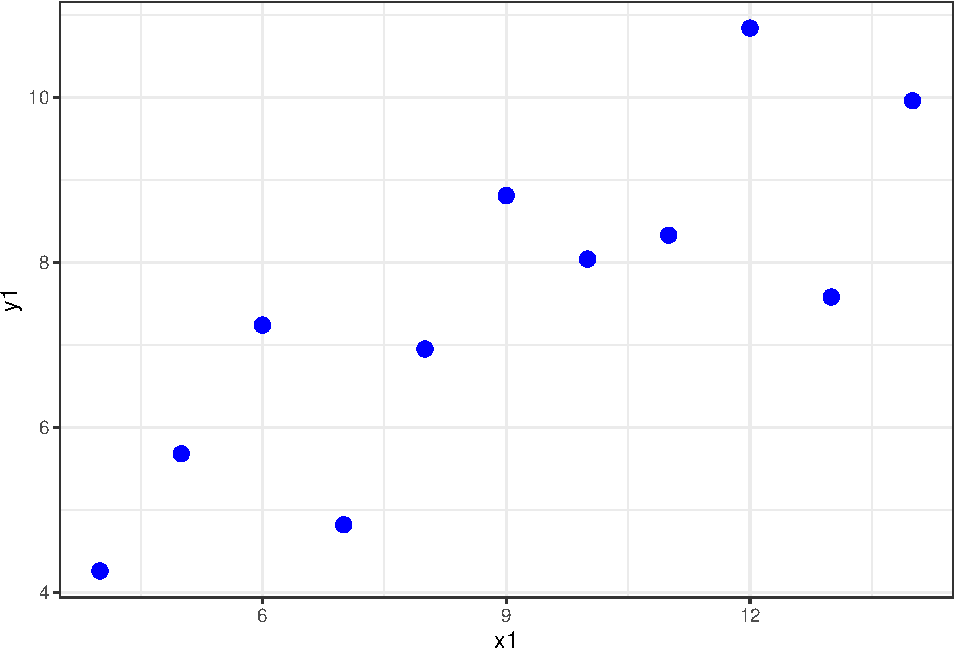
\includegraphics[width=1\linewidth]{007-coding_files/figure-latex/unnamed-chunk-25-1} \end{center}

\begin{Shaded}
\begin{Highlighting}[]
\NormalTok{graph2 <-}\StringTok{ }\KeywordTok{ggplot}\NormalTok{(}\DataTypeTok{data =}\NormalTok{ anscombe, }\DataTypeTok{mapping =} \KeywordTok{aes}\NormalTok{(}\DataTypeTok{x =}\NormalTok{ x2, }\DataTypeTok{y=}\NormalTok{y2))}
\NormalTok{graph2 }\OperatorTok{+}\StringTok{ }\KeywordTok{geom_point}\NormalTok{(}\DataTypeTok{color=}\StringTok{'blue'}\NormalTok{,}\DataTypeTok{size=}\DecValTok{3}\NormalTok{) }\CommentTok{#change this line for different look}
\end{Highlighting}
\end{Shaded}

\begin{center}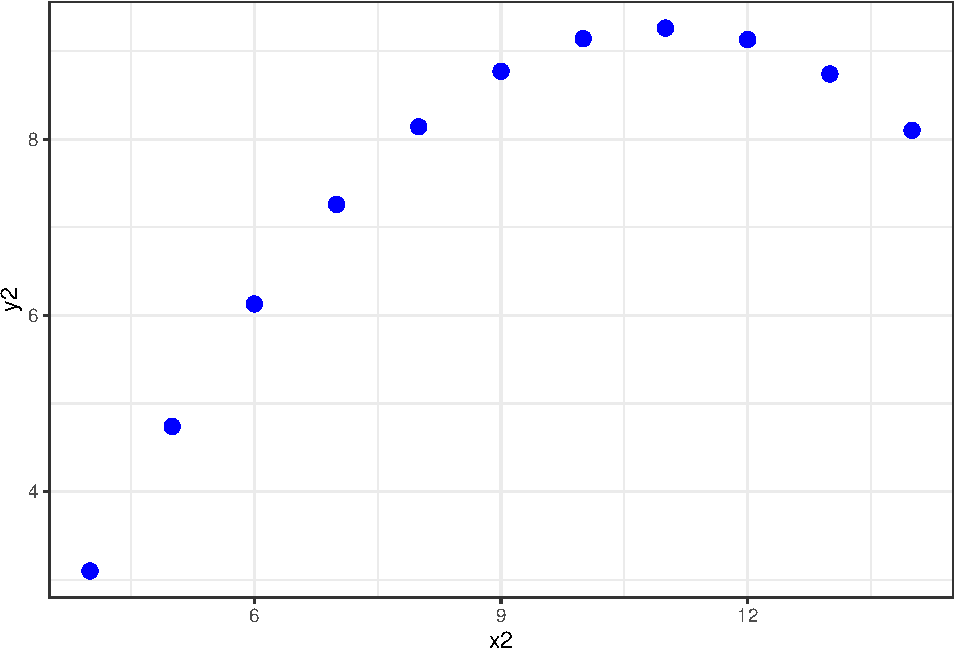
\includegraphics[width=1\linewidth]{007-coding_files/figure-latex/unnamed-chunk-26-1} \end{center}

Adding variables means you only need to edit one line to change the look
of both plots

\begin{Shaded}
\begin{Highlighting}[]
\NormalTok{pointcolour=}\StringTok{'red'}\NormalTok{; pointsize=}\DecValTok{5}\NormalTok{ ; pointshape =}\StringTok{ }\DecValTok{23} \CommentTok{#change this line for different look}

\NormalTok{graph1 <-}\StringTok{ }\KeywordTok{ggplot}\NormalTok{(}\DataTypeTok{data =}\NormalTok{ anscombe, }\DataTypeTok{mapping =} \KeywordTok{aes}\NormalTok{(}\DataTypeTok{x =}\NormalTok{ x1, }\DataTypeTok{y=}\NormalTok{y1)) }
\NormalTok{graph1 }\OperatorTok{+}\StringTok{ }\KeywordTok{geom_point}\NormalTok{(}\DataTypeTok{color=}\NormalTok{pointcolour,}\DataTypeTok{size=}\NormalTok{pointsize, }\DataTypeTok{shape =}\NormalTok{ pointshape) }\CommentTok{# never change these lines}
\end{Highlighting}
\end{Shaded}

\begin{center}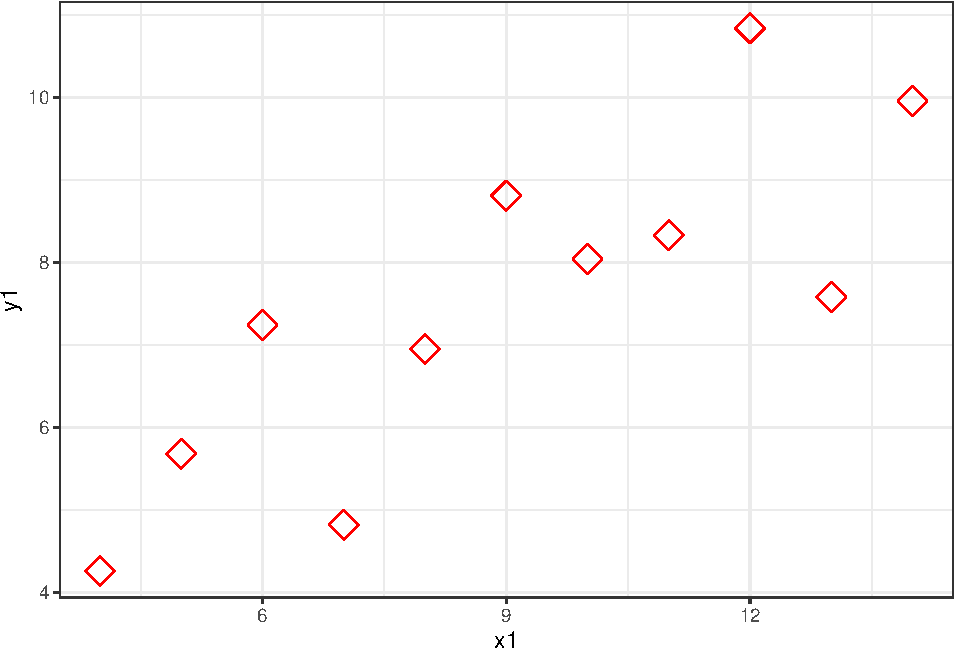
\includegraphics[width=1\linewidth]{007-coding_files/figure-latex/unnamed-chunk-27-1} \end{center}

\begin{Shaded}
\begin{Highlighting}[]
\NormalTok{graph2 <-}\StringTok{ }\KeywordTok{ggplot}\NormalTok{(}\DataTypeTok{data =}\NormalTok{ anscombe, }\DataTypeTok{mapping =} \KeywordTok{aes}\NormalTok{(}\DataTypeTok{x =}\NormalTok{ x2, }\DataTypeTok{y=}\NormalTok{y2))}
\NormalTok{graph2 }\OperatorTok{+}\StringTok{ }\KeywordTok{geom_point}\NormalTok{(}\DataTypeTok{color=}\NormalTok{pointcolour,}\DataTypeTok{size=}\NormalTok{pointsize, }\DataTypeTok{shape =}\NormalTok{ pointshape) }\CommentTok{# never change these lines}
\end{Highlighting}
\end{Shaded}

\begin{center}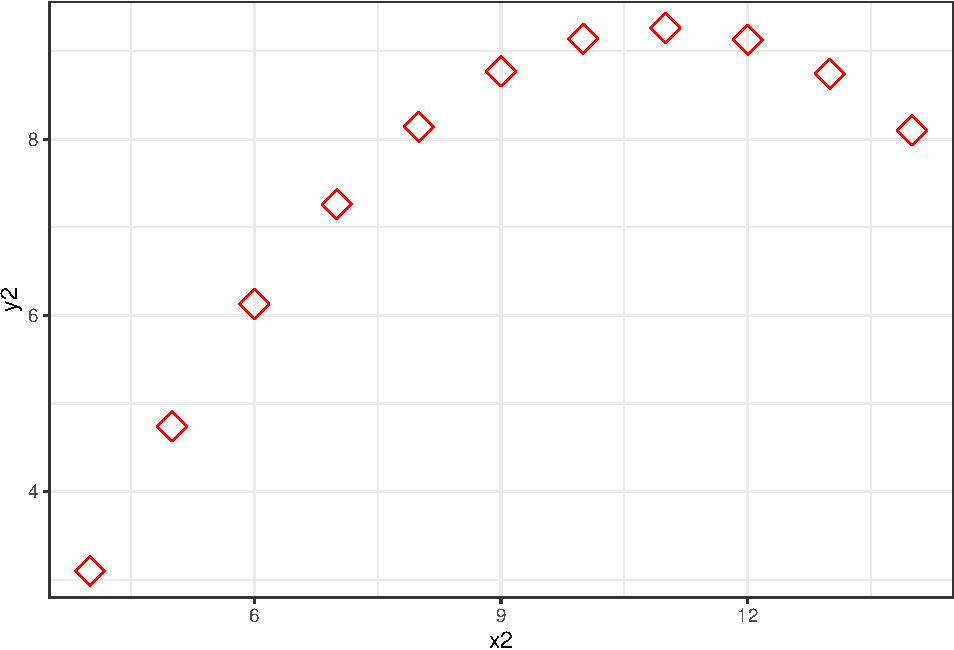
\includegraphics[width=1\linewidth]{007-coding_files/figure-latex/unnamed-chunk-27-2} \end{center}

This may seem minor, but as your code gets longer developing habits like
this will save you time, and make your code easier to work with.

\subsection{Functionalise \& Generalise}\label{functionalise-generalise}

If you ever find yourself using very similar lines of code, you should
think about making a function. Functions make your code shorter and
easier to read (and write), and they make it \emph{way} easier to update
(because when you catch a bug you can just update the code in the
function, rather than every time you repeated those lines).

Functions are also an opportunity to think to yourself ``what is the
most general purpose way of doing what I'm doing''. Thinking like this
will help you develop powerful, flexible, code which you can use to do
multiple things.

Let's look at a toy example:

\begin{Shaded}
\begin{Highlighting}[]
\NormalTok{mynumbers =}\StringTok{ }\KeywordTok{c}\NormalTok{(}\DecValTok{2}\NormalTok{,}\DecValTok{3}\NormalTok{,}\DecValTok{4}\NormalTok{)}

\CommentTok{#double and add one to each number}
\NormalTok{mynumbers[}\DecValTok{1}\NormalTok{] <-}\StringTok{ }\NormalTok{mynumbers[}\DecValTok{1}\NormalTok{]}\OperatorTok{*}\DecValTok{2}\OperatorTok{+}\DecValTok{1} \CommentTok{# line 1}
\NormalTok{mynumbers[}\DecValTok{2}\NormalTok{] <-}\StringTok{ }\NormalTok{mynumbers[}\DecValTok{2}\NormalTok{]}\OperatorTok{*}\DecValTok{2}\OperatorTok{+}\DecValTok{1} \CommentTok{# line 2}
\NormalTok{mynumbers[}\DecValTok{3}\NormalTok{] <-}\StringTok{ }\NormalTok{mynumbers[}\DecValTok{3}\NormalTok{]}\OperatorTok{*}\DecValTok{2}\OperatorTok{+}\DecValTok{1} \CommentTok{# line 3}

\KeywordTok{print}\NormalTok{(mynumbers)}
\end{Highlighting}
\end{Shaded}

\begin{verbatim}
## [1] 5 7 9
\end{verbatim}

This can be improved with a function

\begin{Shaded}
\begin{Highlighting}[]
\NormalTok{myfunc <-}\StringTok{ }\ControlFlowTok{function}\NormalTok{(num)\{}
  \CommentTok{#toy function, doubles and adds 1}
  \KeywordTok{return}\NormalTok{(num}\OperatorTok{*}\DecValTok{2}\OperatorTok{+}\DecValTok{1}\NormalTok{)}
\NormalTok{  \}  }

\NormalTok{mynumbers =}\StringTok{ }\KeywordTok{c}\NormalTok{(}\DecValTok{2}\NormalTok{,}\DecValTok{3}\NormalTok{,}\DecValTok{4}\NormalTok{)}

\NormalTok{mynumbers <-}\StringTok{ }\KeywordTok{myfunc}\NormalTok{(mynumbers) }\CommentTok{# all the work with 1 line!}

\KeywordTok{print}\NormalTok{(mynumbers)}
\end{Highlighting}
\end{Shaded}

\begin{verbatim}
## [1] 5 7 9
\end{verbatim}

This code is easier to read, easier to change, and you can write new
code which uses this function again.

\subsection{Ask for help}\label{ask-for-help}

Nobody finds this easy straight away. Learning how to find help a core
programming skill (along with not giving up when it feels like you are
completely stuck).

Part of this is knowing how programming people talk about stuff so you
can search effectively for solutions.

If you get an error message, copy and paste it into your search.

If you are really stuck, just trying to descibe you problem is a good
way of indentifying exactly what you want to do, and why you can't. When
you've described your problem full - see this
\href{https://stackoverflow.com/questions/5963269/how-to-make-a-great-r-reproducible-example}{How
to make a great R reproducible example} - you can ask a friend or post
it to a forum.

If you're on this module you can post it to Slack on the r-coding
channel, or if not try seeking out R groups in your city or institution.
Shout out to \href{https://rladies.org/}{Rladies}

\subsection{More}\label{more-1}

\begin{itemize}
\tightlist
\item
  \href{https://inattentionalcoffee.wordpress.com/2017/01/13/program-better-for-fun-and-for-profit/}{Program
  better, for fun and for profit}
\item
  \href{https://kkulma.github.io/2018-03-18-Prime-Hints-for-Running-a-data-project-in-R/}{Prime
  Hints For Running A Data Project In R}
\item
  Software Carpentry:
  \href{https://swcarpentry.github.io/r-novice-inflammation/06-best-practices-R/}{Best
  Practices for Writing R Code}
\item
  Nice R code:
  \href{https://nicercode.github.io/intro/bad-habits.html}{bad habits}
\item
  Barnes, N. (2010).
  \href{https://www.nature.com/articles/467753a}{Publish your computer
  code: it is good enough}. Nature, 467(7317), 753-753.
\item
  Axelrod, V. (2014).
  \href{https://www.frontiersin.org/articles/10.3389/fpsyg.2014.01435/full}{Minimizing
  bugs in cognitive neuroscience programming}. Frontiers in psychology,
  5, 1435.
\item
  Wilson, G., Aruliah, D. A., Brown, C. T., Hong, N. P. C., Davis, M.,
  Guy, R. T., \ldots{} \& Waugh, B. (2014).
  \href{http://journals.plos.org/plosbiology/article?id=10.1371/journal.pbio.1001745}{Best
  practices for scientific computing}. PLoS biology{]} 12(1), e1001745.
\end{itemize}

\chapter{Rmarkdown}\label{rmarkdown}

These pages are written in Rmarkdown. You can see this individual file
\href{https://github.com/tomstafford/psy6422/blob/master/008-rmarkdown.Rmd}{here
in the online repositry}

Rstudio magic turns this file in to a webpage which you are probably
looking at now.

Compare the file and the webpage.

\textbf{In the webpage this line is in bold. Why?}

\emph{In the webpage this line is in italic. Why?}

\section{And this line is a heading}\label{and-this-line-is-a-heading}

\chapter{Git and Github}\label{git-and-github}

With our guest lecturer, Seb James

\section{Before the class}\label{before-the-class}

Create an account on \href{https://github.com/}{github.com}, if you
don't already have one.

Make sure you have access to git on your computer:

\begin{itemize}
\tightlist
\item
  Students using windows can install: \url{https://gitforwindows.org/}
  Once installed they should be able to open a git bash window and type
  \texttt{git\ -\/-version}
\item
  Students on a Mac will have git if they install `Xcode' and `Command
  line tools for Xcode'.They can test by opening a terminal and typing
  \texttt{git\ -\/-version}
\end{itemize}

\section{Resources}\label{resources}

Intro to git talk: \url{https://github.com/ABRG-Models/GitTutorial}

Software carpentry: \url{http://sebjameswml.github.io/git-novice/}

\section{Bonus Links}\label{bonus-links}

\href{https://www.sbf5.com/~cduan/technical/git/}{Understanding Git
Conceptually}

Vuorre, M., \& Curley, J. P. (2018).
\href{https://journals.sagepub.com/doi/full/10.1177/2515245918754826}{Curating
research assets: A tutorial on the git version control system}. Advances
in Methods and Practices in Psychological Science, 1(2), 219-236.

\chapter{Publishing}\label{publishing}

\section{Sharing your Rmd files via Github
pages}\label{sharing-your-rmd-files-via-github-pages}

\begin{enumerate}
\def\labelenumi{\arabic{enumi}.}
\item
  Save your analysis in a file \texttt{index.Rmd}
\item
  Click `knit' in RStudio
\end{enumerate}

\begin{itemize}
\tightlist
\item
  (selecting `knit to HTML' if you haven't specified this in the header)
\end{itemize}

\begin{enumerate}
\def\labelenumi{\arabic{enumi}.}
\setcounter{enumi}{2}
\item
  Save your files to a github repo:
  \texttt{https://github.com/username/myrepo/}
\item
  Via the browser, edit the settings for the repo and scroll down to
  `Github Pages'. There change `Source' to `Master'
\end{enumerate}

Your pages will be at \url{https://username.github.io/myrepo/}

\section{Other sharing options}\label{other-sharing-options}

OSF

Jupyter notebooks

\chapter{Advanced Topics}\label{advanced-topics}

\section{Better graphs}\label{better-graphs}

\section{Reproducibility}\label{reproducibility}

\url{https://luisdva.github.io/rstats/annotater/}

\section{Preview of other advanced
topics}\label{preview-of-other-advanced-topics}

\appendix


\chapter{Extra Reading}\label{extra-reading}

Further reading, including books, links, demos and packages. You don't
need to read all of this, but you will want to dig around. If I could
recommend one book to accompany the courseit would be

\begin{info}
Healy, K. (2018). \href{https://socviz.co/}{Data visualization: a
practical introduction}. Princeton University Press.
\end{info}

\section{Visualisation (theory)}\label{visualisation-theory}

Healy, K. (2018). \href{https://socviz.co/}{Data visualization: a
practical introduction}. Princeton University Press.

Cairo, A. (2012). The Functional Art: An introduction to information
graphics and visualization. New Riders.

Tufte, E. R. (2001). The visual display of quantitative information.
Cheshire, CT: Graphics press.

McCandless, D. (2012). Information is beautiful. London: Collins.

Rougier, N. P., Droettboom, M., \& Bourne, P. E. (2014). Ten simple
rules for better figures. PLoS Comput Biol, 10(9), e1003833.
\url{https://journals.plos.org/ploscompbiol/article?id=10.1371/journal.pcbi.1003833}

Weissgerber, T. L., Milic, N. M., Winham, S. J., \& Garovic, V. D.
(2015).
\href{https://journals.plos.org/plosbiology/article?id=10.1371/journal.pbio.1002128}{Beyond
bar and line graphs: time for a new data presentation paradigm}. PLoS
biology, 13(4).

\section{The Reproducibility Crisis}\label{the-reproducibility-crisis}

Cancer Biology Reproducibility Project
\url{https://www.enago.com/academy/the-reproducibility-project-cancer-biology-to-replicate-only-18-studies-now/}

Economics reproducibility
\url{https://www.wired.com/story/econ-statbias-study/}

Video: Is Most Published Research Wrong
\url{https://www.youtube.com/watch?v=42QuXLucH3Q}

Demo: p-hacking
\url{https://fivethirtyeight.com/features/science-isnt-broken/\#part1}

Open Science Collaboration. (2015). Estimating the reproducibility of
psychological science. Science, 349(6251), aac4716.

\section{Better practice}\label{better-practice}

Munafo, M. R., et al. (2017). A manifesto for reproducible science .
Nature Human Behaviour, 1, 0021. DOI: 10.0138/s41562-016-0021.

Markowetz, F. (2015). Five selfish reasons to work reproducibly. Genome
biology, 16(1), 274.
\url{https://genomebiology.biomedcentral.com/articles/10.1186/s13059-015-0850-7}

A Guide to Reproducible Code in Ecology and Evolution
\url{https://www.britishecologicalsociety.org/wp-content/uploads/2017/12/guide-to-reproducible-code.pdf}

Gael Varoquaux: Computational practices for reproducible science
\url{https://www.slideshare.net/GaelVaroquaux/computational-practices-for-reproducible-science}

``our wishlist for what knowledge and skills we'd find in a
well-prepared data scientist candidate coming from a masters program.''
\url{https://github.com/brohrer/academic_advisory/blob/master/curriculum_roadmap.md}

\section{Project organisation}\label{project-organisation-1}

Mike Frank onboarding guide
\url{http://babieslearninglanguage.blogspot.co.uk/2017/01/onboarding.html}

Jenny Bryan: Naming Things
\url{http://www2.stat.duke.edu/~rcs46/lectures_2015/01-markdown-git/slides/naming-slides/naming-slides.pdf}

Broman \& Woo (2017) Data Organization in Spreadsheets
\url{https://www.tandfonline.com/doi/full/10.1080/00031305.2017.1375989}

Video: Data Sharing and Management Snafu in 3 Short Acts
\url{https://www.youtube.com/watch?time_continue=2\&v=N2zK3sAtr-4}

Hadley Wickham: Tidy Data:
\url{http://vita.had.co.nz/papers/tidy-data.pdf}

\section{Coding}\label{coding}

Readings in Applied Data Science
\url{https://github.com/hadley/stats337\#readings}

Stack overflow: asking good questions
\url{https://stackoverflow.com/help/how-to-ask}

Stack overflow: provide a minimal, complete, verifable example
\url{https://stackoverflow.com/help/mcve}

Our Software Dependency Problem \url{https://research.swtch.com/deps}

From Psychologist to Data Scientist
\url{https://www.neurotroph.de/2019/01/from-psychologist-to-data-scientist/}

Bret Victor:
\href{http://worrydream.com/LearnableProgramming/}{Learnable
Programming: Designing a programming system for understanding programs}

\href{https://www.kdnuggets.com/2019/04/top-10-coding-mistakes-data-scientists.html}{Top
10 Coding Mistakes Made by Data Scientists}

\section{R}\label{r}

{[}Prime Hints For Running A Data Project In{]}
R(\url{https://kkulma.github.io/2018-03-18-Prime-Hints-for-Running-a-data-project-in-R/})

Grolemund, G., \& Wickham, H. (2018). R for data science. * See also
\url{https://r4ds.had.co.nz/}

Getting Used to R, RStudio, and R Markdown
\url{https://rbasics.netlify.com/}

Adler, J. (2010). R in a nutshell: A desktop quick reference. " O'Reilly
Media, Inc.``.

Intro to R (Liz Page-Gould): \url{http://www.page-gould.com/r/uoft/}

Open R Textbook (Danielle Navarro):
\url{http://health.adelaide.edu.au/psychology/ccs/teaching/lsr/}

\begin{itemize}
\tightlist
\item
  Particularly chapter 3
  \url{https://learningstatisticswithr-bookdown.netlify.com/intror}
\end{itemize}

RStudio Cheat Sheets:
\url{https://www.rstudio.com/resources/cheatsheets/}

Here::Here \url{https://github.com/jennybc/here_here}

\url{https://swirlstats.com/}

Lisa DeBruine, \& Dale Barr. (2019). Data Skills for Reproducible
Science. Zenodo. \url{doi:10.5281/zenodo.3564348}
\url{https://psyteachr.github.io/msc-data-skills/}

\section{Making graphs (practice)}\label{making-graphs-practice}

Graphing in R (Eric-Jan Wagenmakers and Quentin F. Gronau):
\url{http://shinyapps.org/apps/RGraphCompendium/index.php}

\url{https://gupsych.github.io/data_skills/03_ggplot.html}

\chapter{Notes}\label{notes}

\section{Credit}\label{credit}

These pages based on \href{https://psyteachr.github.io/book-template/}{a
template} published by the awesome
\href{https://psyteachr.github.io/about/}{psyTeachR team}. Extra thanks
to Lisa DeBruine for help.

Find the repo here: \url{https://github.com/tomstafford/psy6422/}

\section{Python}\label{python}

This course teaches general principles of coding and computation, and
specific skills for data management and visualisation in R. Lots of
people in the data science world, particularly in areas which align with
computer science / machine learning, use Python.

I decided to teach this course in R because the community around a
language is as important as the language. You can do anything in any
language, and most things as easily in Python as in R, but
Psychologists, biologists and scholars from across the social sciences
tend to use R, so I'm teaching this course in R.

If you want to learn Python, I recommend:

\begin{itemize}
\tightlist
\item
  Resource list:
  \href{https://wiki.python.org/moin/BeginnersGuide/NonProgrammers}{Python
  for Non-Programmers}
\item
  Pages \href{https://realpython.com/start-here/}{RealPython: Learn
  Python Programming, By Example}
\item
  Book:
  \href{https://jakevdp.github.io/PythonDataScienceHandbook/}{Python
  Data Science Handbook} by Jake VanderPlas
\item
  Book: \href{https://wesmckinney.com/pages/book.html}{Python for Data
  Analysis} by Wes McKinney
\item
  Pages: \href{https://chrisalbon.com/}{chrisalbon.com}
\item
  Pages: \href{https://towardsdatascience.com}{TowardsDataScience}, for
  example this one
  \href{https://towardsdatascience.com/a-quick-introduction-to-the-pandas-python-library-f1b678f34673}{A
  Quick Introduction to the ``Pandas'' Python Library}
\item
  Book: \href{http://www.pygaze.org/pep/}{Python for Experimental
  Psychologists} by Edwin Dalmaijer
\item
  Pages: \href{https://www.w3schools.com/python/default.asp}{w3Schools}
\end{itemize}

\section{General righteousness}\label{general-righteousness}

You should use a password manager. Really.
\href{https://www.lastpass.com}{LastPass} is recommended

You should know how to use a VPN

\begin{itemize}
\tightlist
\item
  Advice for Sheffield students here:
  \href{https://www.sheffield.ac.uk/it-services/remote/students}{Working
  remotely - information for students}
\item
  You can test by visiting
  \href{https://journals.sagepub.com/doi/full/10.1177/0956797613511466}{this
  page}. If you are in the University network (either on campus or via a
  VPN) it will offer you the chance to download the article PDF.
  Otherwise it will try and charge you \$35 for the privilege.
\end{itemize}

\section{Testimonials}\label{testimonials}

\href{https://www.sheffield.ac.uk/psychology/prospectivepg/masters/stories/peter-carr-1.817457}{Peter
Carr}

This is the first year the
\href{https://www.sheffield.ac.uk/psychology/prospectivepg/masters/data-science}{MSc
in Psychological Research Methods with Data Science} has run, so more
soon!

\bibliography{book.bib,packages.bib}

\end{document}
